\section{Entanglement in front of a thermal shield}\label{sec:5:thermal-entanglement}
The entanglement generation between the two particles depends heavily on the variation of the separation between the shield and the particles, as has been seen in \cref{cha:entanglement-generation}.
The vibrating shield can be interpreted as varying the separation and angle of the cat-state in front of the plate - visualized in \cref{fig:5:vibrating-translation-to-variations}.
\begin{figure}[!htbp]
  \centering
  \def\svgwidth{\textwidth}
  \input{./../figures/plate-vibration.pdf_tex}
  \caption{For a large $r_s \gg R$ and locally flat shield, the thermal vibrations with amplitude $z$ can be interpreted as a static shield where the particle $A$ (shown in the figure) is placed at $L+\Delta L$ at angle $\theta$ and particle $B$ is places at $L-\Delta L$ with angle $-\theta$ where both variations depend on the amplitude. At low vibrational frequencies $1/\omega \approx t_\mathrm{max}$ the amplitude can be assumed to be static during a experimental run and for each measurement thermally distributed around $\mean{z}=0$ with $\Delta z$ given by eq. \eqref{eq:5:amplitude-variance}.}
  \label{fig:5:vibrating-translation-to-variations}
\end{figure}
This is only a good approximation for shields larger than the particles radius $r_s \gg R$ and low vibrating frequencies $1/\omega \approx t_\mathrm{max}$ and can therefore be used well to describe the highly disturbing first few modes on a large shield.
Furthermore, this interpretation is possible because as shown in \cref{sec:3:imperfect-plates}, the Casimir interaction between a sphere and a tilted plane does not differ from the interaction between a flat plane.
Contrary to the problem considered in \cref{cha:entanglement-generation}, here only the thermal amplitude $z_{kl}$ is a independent random variable distributed around $\mean{z_{kl}} = 0$ with standard deviation $\Delta z_{kl}$ given by eq. \eqref{eq:5:amplitude-variance}. 
Both, the variations in the particle-shield separation $\Delta L$ as well as in the angle $\theta$ are correlated to the amplitude $z$.
For a large shield, this can be understood as
\begin{equation}
  \theta = \arctan(z \abs{\nabla u}) \approx z \abs{\nabla u} \quad \text{and} \quad \Delta L = z \abs{u}
\end{equation}
where $\nabla u$ is the gradient of the shape of the vibrational mode.
Performing similar calculations as done before in \cref{cha:entanglement-generation}, the averaged density matrix $\mean{\rho}$ dependent on $\Delta z_{kl}$ can be calculated and is given in \cref{apx:density-matrix-vibrating-plate}.
The entanglement quantified by the logarithmic negativity dependent on the temperature $T$ and on the particle-shield separation $L$ is given by eq. \eqref{eq:apx:en-thermal-shield} and is shown in \cref{fig:5:entanglement-temperature}.
\begin{figure}[!htbp]
  \centering
  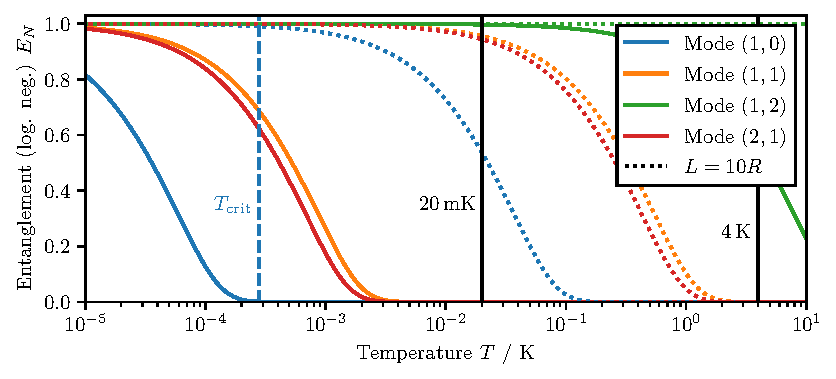
\includegraphics[width=\textwidth]{./../figures/vibrations/log-neg-shield-vibrations-T.pdf}
  \caption{Entanglement between the particles (parallel orientation) in front of a thermal shield at different temperature $T$ for selected modes. At a temperature $T_\mathrm{crit,\,kl}$, all entanglement is lost if the mode $(k,l)$ is present. This critical point shifts with higher separation distance $T_\mathrm{crit}\propto L^4$}
  \label{fig:5:entanglement-temperature}
\end{figure}
At reasonable temperatures, entanglement in the presence the mode $(1,0)$ is in theory only observable for large separations.
In fact, the dependence of the critical temperature $T_\mathrm{crit}$ on the separation $L$ is known as for large separation in the LSL the following is expected:
\begin{equation}
  T_\mathrm{crit} \sim (\Delta z_\mathrm{crit})^2 \sim \left(\frac{L^5}{t_\mathrm{max}} \right)^2 \sim L^4 .
\end{equation}
The required large separations are not surprising considering that the thermal amplitudes $\Delta z_{1,0} \approx 9 \times 10^{-11}\si{m}$ at $20\si{mK}$ are comparable with the previously calculated values the variation in the shield-particle separation $\Delta L_\mathrm{crit}$ in \cref{cha:entanglement-generation}.
Interestingly this result does not change for different shield radii - at least as long as the condition $r_s \gg R$ is fulfilled and the shape of the vibrational mode can locally be linearized.
This is because the gradient $\abs{\nabla u} \propto 1/r_s$ perfectly cancels with the dependence on $z \propto r_s$ leaving $\theta$ independent of $r_s$. 
If the cat-state orientation is now chosen parallel to the shield, the dependence on $\Delta L$ is irrelevant leaving the final resulting entanglement independent of $r_s$.
However, as seen in \cref{fig:5:entanglement-temperature}, the mode number $(k,l)$ has a huge effect on the entanglement generation. Higher modes correspond to higher vibrational frequencies and thus smaller amplitudes $\Delta z$.
Asymptotically, a scaling of $T_\mathrm{crit}$ in the order of $\mathcal{O}(k^2 + l^2)$ is expected.
\begin{figure}[!htbp]
  \centering
  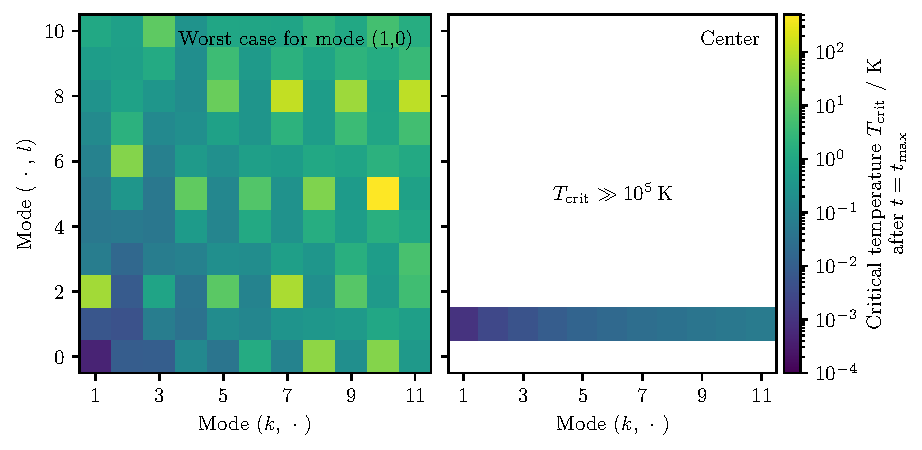
\includegraphics[width=\textwidth]{./../figures/vibrations/T-crit-modes.pdf}
  \caption{Critical temperature $T_\mathrm{crit}$, at which no entanglement is measurable anymore for different modes at a separation of $L = 2R = 2\si{\mu m}$. The shape of the vibrational modes is considered. The particle is either placed at the position of the highest gradient of mode $(1,0)$ (\textbf{left}) or in the center of the shield (\textbf{right}).}
  \label{fig:5:T-crit-modes}
\end{figure}
It becomes evident, that only the first couple of modes are actually relevant as all others do not destroy entanglement up to temperatures much higher than necessary.



\subsection{Analytic dynamics}
The influence of the thermal shield on entanglement generation can be calculated analytically. 
The Hamiltonian which governs the mutual interaction of the two particles and between each particle and the thermal shield is given by
\begin{align}\label{eq:5:hamiltonian}
  \begin{split}
    \op{H} = \sum_{\substack{m\in\{(k,l)\}\\ k \geq 1,\ l \geq 0}} \biggl\{ & \hbar \omega_m \left(\op{a}^\dagger_m \op{a}_m + \frac{1}{2}\right) \\
    &+ g^{(1)}_\mathrm{A,m,Cas}(\op{a}_m + \op{a}^\dagger_m) \left( \ketbra{\psi^{(1)}_A} \otimes \identity \right)
     + g^{(2)}_\mathrm{A,m,Cas}(\op{a}_m + \op{a}^\dagger_m) \left( \ketbra{\psi^{(2)}_A} \otimes \identity \right) \\
    &+ g^{(1)}_\mathrm{B,m,Cas}(\op{a}_m + \op{a}^\dagger_m) \left( \identity \otimes \ketbra{\psi^{(1)}_B} \right)
     + g^{(2)}_\mathrm{B,m,Cas}(\op{a}_m + \op{a}^\dagger_m) \left( \identity \otimes \ketbra{\psi^{(2)}_B} \right)\biggr\} \\
    + g^{(1,1)}_\mathrm{Grav}&\ketbra{\psi^{(1)}_A \psi^{(1)}_B} + g^{(1,2)}_\mathrm{Grav}\ketbra{\psi^{(1)}_A \psi^{(2)}_B} \\
    + g^{(2,1)}_\mathrm{Grav}&\ketbra{\psi^{(2)}_A \psi^{(1)}_B} + g^{(2,2)}_\mathrm{Grav}\ketbra{\psi^{(2)}_A \psi^{(2)}_B}
  \end{split}
\end{align}
where 
\begin{equation}
  g^{(ij)}_\mathrm{Grav} = \frac{G M^2}{L^{(ij)}}
\end{equation}
is the gravitational coupling between the states $\ket{\psi^{(i)}_A}$ and $\ket{\psi^{(j)}_B}$ separated by $L^{(ij)}$ from eq. \eqref{eq:4:L-gravity}.
This interaction is similar to the ones considered in \cref{cha:entanglement-generation}, as it is independent of the shields movement.
The gravitational coupling between the shield and the particles have been neglected here, as this coupling is by a factor $10^{7}$ times weaker than the Casimir interaction, as calculated in \cref{subsec:5:shield-gravitation}.
This interaction between state $\ket{\psi_{A(B)}^{(i)}}$ and the shield is denoted by $\tilde{g}^{(i)}_\mathrm{A(B),\,m,\,Cas}$. These couplings are dependent on the amplitude $\op{z}_{m} = \sqrt{\hbar/2\tilde{m}\omega_m} (\op{a}_m + \op{a}^\dagger_m)$ and the shape $u_{m}(r_{A(B)})$ of the vibrational mode $m\in\{(k,l)\}$ at the position $r^{(i)}_{A(B)}$ of the cat state:
\begin{equation}
  \tilde{g}^{(i)}_\mathrm{A(B),\,m,\,Cas} = \frac{\hbar c \pi^3}{720} \left(\frac{\varepsilon_r - 1}{\varepsilon_r + 1}\right)\varphi(\varepsilon_r) \frac{R}{(\mathscr{L} + \op{z}_m u_m(r))^2} \approx g_\mathrm{PFA} \left(\frac{1}{\mathscr{L}^2} + \frac{2 \op{z}_m u_m(r^{(i)}_{A(B)})}{\mathscr{L}^3}\right) .
\end{equation}
Ignoring the first term in the expansion, which just produces a global phase in the evolved system, the couplings $g_\mathrm{Cas}$ appearing in eq. \eqref{eq:5:hamiltonian} are ultimately given by
\begin{equation}
  g^{(i)}_\mathrm{A(B),\,m,\,Cas} = g_\mathrm{PFA} \frac{2u_m(r^{(i)}_{A(B)})}{\mathscr{L}^3} \sqrt{\frac{\hbar}{2 \tilde{m} \omega_m}} .
\end{equation}
It is possible to analytically calculate the dynamics of the two particles in delocalized cat-states $\rho_\mathrm{system}$ in front of the thermal shield.
The initial state is given by
\begin{equation}
  \rho_0 = \bigotimes_{m\in\{(k,l)\}} \left(\rho_\mathrm{th,\,m}\right) \otimes \rho_\mathrm{system}
\end{equation}
where $\rho_\mathrm{system}$ is given by eq. \eqref{eq:2:initial-state} and $\rho_\mathrm{th,m}$ is the thermal state of the vibrational mode $m$, which is expressible in the number basis $\left\{\ket{n}\right\}$ and in the coherent state basis $\left\{\ket{\alpha}\right\}$ as \cite{Steiner_2024}
\begin{equation}
  \rho_\mathrm{th,m} = \frac{1}{Z} \sum_{n=1}^{\infty} e^{-\beta \hbar \omega_m (n + 1/2)} \ketbra{n} = \int \dd \alpha^2 \frac{1}{\pi \bar{n}} e^{-\frac{\abs{\alpha}^2}{\bar{n}}} \ketbra{\alpha} .
\end{equation}
Here, $Z = \tr e^{-\beta \hbar \omega_m (\op{n}+1/2)} = e^{-\beta \hbar \omega_m/2}/(1-e^{-\beta \hbar \omega_m})$ is the partition function and $\bar{n} = 1/(e^{\beta \hbar \omega_m} - 1)$ is the average thermal occupation number at temperature $T$. 
The system of the evolved particles after time $t$ is given by tracing out the thermal shield as
\begin{equation}
  \rho_\mathrm{system}(t) = \tr_\mathrm{th} \left( \op{U}(t) \rho_0 \op{U}^\dagger(t) \right)  
\end{equation}
and is computed in \cref{apx:thermal-shield-time-evolution}. It can be expressed in the form
\begin{equation}
  \rho_\mathrm{system}(t) = \frac{1}{4} \begin{pmatrix}
    1 & e^{i\phi_{11,12}} e^{-\gamma_{11,12}} & e^{i\phi_{11,21}} e^{-\gamma_{11,21}} & e^{i\phi_{11,22}} e^{-\gamma_{11,22}} \\
    & 1 & e^{i\phi_{12,21}} e^{-\gamma_{12,21}} & e^{i\phi_{12,22}} e^{-\gamma_{12,22}} \\
    & & 1 & e^{i\phi_{21,22}} e^{-\gamma_{21,22}} \\
    & & & 1 \\
  \end{pmatrix}
\end{equation}
with the decoherence terms
\begin{equation}\label{eq:5:analytical-decoherence}
  \gamma_{ii',jj'} = \sum_m \frac{4}{\hbar^2\omega_m^2} \abs{(g^{(i)}_{A,m,Cas} + g^{(i')}_{B,m,Cas}) - (g^{(j)}_{A,m,Cas} + g^{(j')}_{B,m,Cas})}^2 \sin^2\left(\frac{\omega_m t}{2}\right) \left[\bar{n} + \frac{1}{2}\right]
\end{equation}
and the phases (where the gravitational part is already given by eq. \eqref{eq:2:evolved-state})
\begin{multline}\label{eq:5:analytical-phases}
  \phi_{ii',jj'} = \sum_m \frac{1}{\hbar} \left( g^{(ii')}_\mathrm{Grav} - g^{(jj')}_\mathrm{Grav} \right) t \\
  + \frac{\sin(\omega_m t)+\omega_m t}{\hbar^2\omega_m^2}\left[(g^{(i)}_{A,m,Cas} + g^{(i')}_{B,m,Cas})^2 - (g^{(j)}_{A,m,Cas} + g^{(j')}_{B,m,Cas})^2\right] .
\end{multline}
It is interesting to see, that even for $T=0$, the decoherence terms $\gamma$ are non-zero. The effect however is only noticeable if the coupling strength $g_\mathrm{Cas}$ is very large, i.e. for small separations $L \approx R$.
The decoherence terms are proportional to $\gamma \propto \omega_m^{-4}$ from which follows an asymptotic dependence on the modes as $\mathcal{O}(k^{-8}+l^{-8})$.
It is therefore asymptotically possible to estimate the combined effect of the first $N$ modes as
\begin{equation}
  \sim \frac{1}{\zeta(8)} \sum_{n=1}^{N} \frac{1}{n^8}
\end{equation}
where $\zeta$ is the Riemann zeta function. The underestimation made, by only considering a few low modes numerically is therefore negligibly small.
Generally, the term $\sin^2(\omega_m t / 2)$ in eq. \eqref{eq:5:analytical-decoherence} is zero for specific times $t = 2 \pi k / \omega_m,\ k\in\mathbb{N}$ depending on the mode $m$. At these times, no decoherence due to mode $m$ is expected and the total entanglement should be similar to the ideal scenario without the shield. This behavior is perfectly captured in \cref{fig:5:entanglement-time-single-mode} and aligns with similar findings from Ref. \cite{Pedernales_2022}.
\begin{figure}[!htbp]
  \centering
  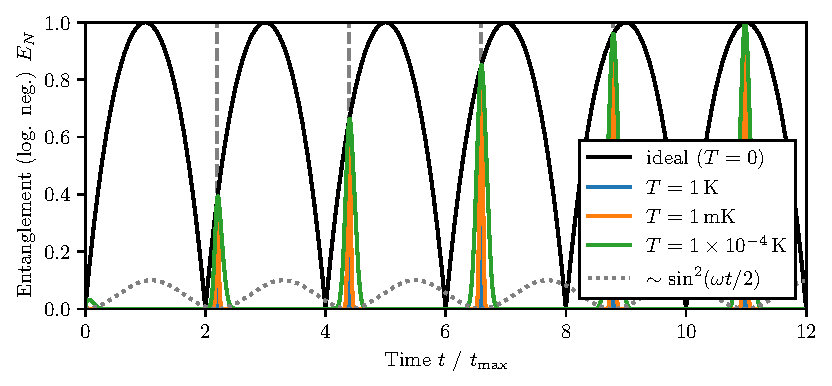
\includegraphics[width=\textwidth]{./../figures/vibrations/entanglement-hamiltonian.pdf}
  \caption{Entanglement dynamics in front of a thermal shield in mode $(1,0)$ at different temperatures. Only at specific times $2\pi k / \omega_{1,0},\ k\in\mathbb{N}$, entanglement is observable. This behavior is expected and aligns with the findings in Ref. \cite{Pedernales_2022}.}
  \label{fig:5:entanglement-time-single-mode}
\end{figure}
The full width at half maximum (FWHM) of the observed peaks at $t=2\pi k/\omega_m$ is approximately given by
\begin{equation}
  \mathrm{FWHM} \approx \frac{4}{\omega}\sqrt{\frac{\log 2}{\gamma}} \propto \frac{1}{\sqrt{\bar{n}}}
\end{equation}
so for high temperatures, entanglement is only measurable in a very short window of time around $2\pi k / \omega_m$.
The effect of multiple modes can also be computed numerically. The resulting decoherence is a sum of all individual modes and the effect of each mode decays rapidly with increasing mode number.
It becomes evident, that at no point in time, the full ideal amount of entanglement can be reached as the frequencies $\omega_i / \omega_j \notin \mathbb{Q}$ for $i \neq j$ \footnote{This is not strictly mathematically proven here, but the fact that the zeros of linear combinations of Bessel functions are transcendental \cite{Lorch_1995} makes this argument likely true. Additionally, it holds that $\omega_{1,0}/\omega_{1,1}\notin\mathbb{Z}$, which on its own is enough to show quasi-periodicity.} and thus the summation of sinusoidal functions with frequencies $\omega_m$ results in a quasi-periodic function that does never repeat exactly and generally never reaches zero.
The combined effect on the entanglement generation between the spheres in the presence of the first 50 vibrational modes is shown in \cref{fig:5:entanglement-multiple-modes} .
\begin{figure}[!htbp]
  \centering
  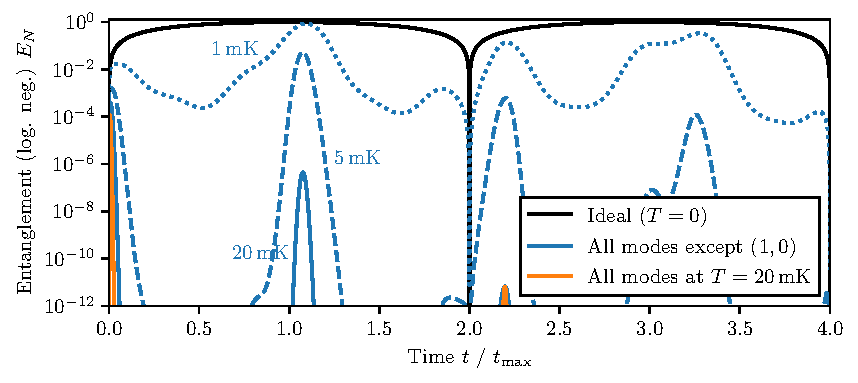
\includegraphics[width=\textwidth]{./../figures/vibrations/entanglement-multiple-modes.pdf}
  \caption{Entanglement dynamics in front of a thermal shield. In orange, the first 50 modes have been used in the numeric calculation. The effect of all remaining modes is around $1.7 \times 10^{-11}\,\%$. In blue, all modes except the first mode $(1,0)$ have been considered at different temperatures ranging vom $1\si{mK}$ up to $20\si{mK}$. The particle-shield separation is fixed at $L = 2R = 20\si{\mu m}$.}
  \label{fig:5:entanglement-multiple-modes}
\end{figure}
This figure additionally also illustrates the overpowering effect of the first mode $(1,0)$.
Entanglement is therefore realistically only measurable at time $t = 2 \pi/\omega_{1,0}$.
But even for temperatures as low as $20\si{mK}$, almost no entanglement is observable, at least for small particle-shield separations.
By increasing the separation distance, the coupling between the shield and the particle due to Casimir interactions decreases with $g_\mathrm{Cas} \propto \mathscr{L}^{-3}$ and thus the coherences aren't destroyed immediately. 
Simultaneously, the gravitational interaction between the particles decreases as well and thus the entanglement generation slows down with $t_\mathrm{max} \propto L^{3}$.
The combined effect on is therefore quantitatively given by $\gamma \propto g_\mathrm{Cas}^2 \sin^2(t) \propto L^{-6} \sin^2(L^3) \xrightarrow{L \gg R} 0$.
In \cref{fig:5:entanglement-thermal-shield-L} the dependence of the entanglement on the particle-shield separation at two specific points in time is shown.
\begin{figure}[!htbp]
  \centering
  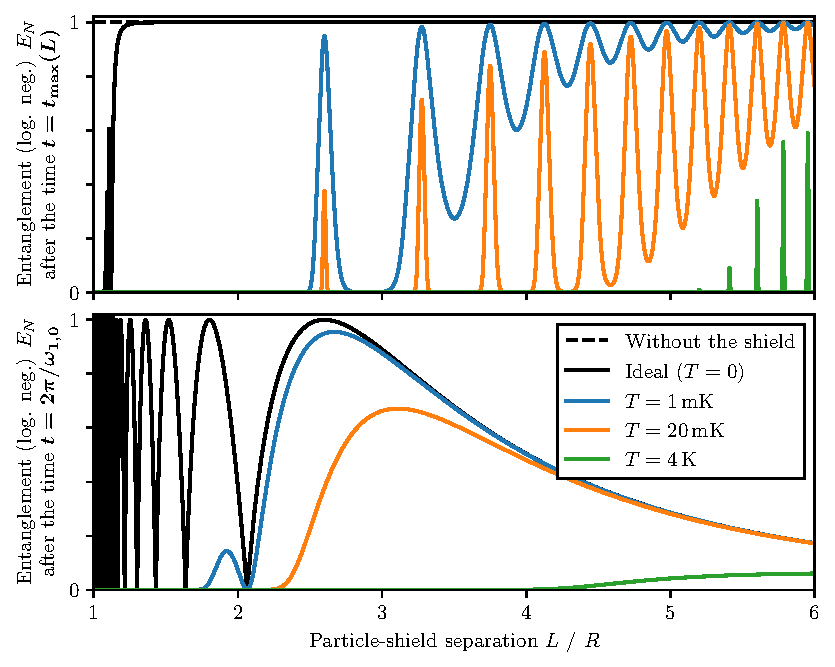
\includegraphics[width=\textwidth]{./../figures/vibrations/all-modes-entanglement-L.pdf}
  \caption{Entanglement for different particle-shield separations $L > R$ at time $t_\mathrm{max}(L)$ (\textbf{top}) and $t_2\pi/\omega_{1,0}\approx 576\si{ms}$ (\textbf{bottom}). The entanglement was calculated at different temperatures for particle and shield parameters given in \cref{tab:paramters}.}
  \label{fig:5:entanglement-thermal-shield-L}
\end{figure}
By measuring at time $t_\mathrm{max}$, ideally without the shield a maximally entangled state is observed. The time $2\pi/\omega_{1,0} = \mathrm{const.}$ stays unchanged by increasing $L$, but $t_\mathrm{max}$ increases resulting in specific separations (e.g. $L \approx 2.6R$ where the measuring time $t_\mathrm{max}$ aligns with $2\pi/\omega_{1,0}$), where entanglement can be measured for the specified time.
By further increasing the separation, the decoherence elements eq. \eqref{eq:5:analytical-decoherence} decrease further resulting in more entanglement even at higher temperatures.
By measuring at the time where the effect of the first mode $(1,0)$ is almost zero, i.e. $2\pi/\omega_{1,0}$, more entanglement can also be observed by increasing the particle-shield separation, as can be seen in \cref{fig:5:entanglement-thermal-shield-L}. However, due of the constant time $2\pi/\omega_{1,0} \approx 576\si{ms}$, at larger separations, the maximally amount of entanglement decreases because the entanglement-generation due to gravity gets slower.
Contrary to above, the radius of the plate has a large effect on the resulting logarithmic negativity. 
The dephasing terms $\gamma \propto \sin^2(\omega) 1/\omega_m^2$ decreases and oscillates rapidly for small shield radii, i.e. large frequencies.
The time between points where the effect of the first mode are almost zero (that is every $\Delta t = 2\pi/\omega_{1,0}$), decreases for smaller shields, making entanglement measurable at almost any point in time.
Numeric calculations show, that even for shields as large as $r_s = 5\si{mm}$, entanglement of around $E_N \approx 0.5$ can be measured at $T = 20\si{mK}$ at close separations (see \cref{fig:apx:entanglement-thermal-shield-rs-5mm}). 

By examining the phases $\phi_{ii',jj'}$, it becomes evident, that similarly to the gravitational force, the Casimir interaction between the particle and the shield can entangle both particles.
Both particles couple to the shield via Casimir interactions, which indirectly lets them interact.
The amount of entanglement however is very small, which can be seen by comparing the phases in eq. \eqref{eq:5:analytical-phases}, where the indirect entanglement depends on $1/\hbar^2$.
Nevertheless it could be potentially problematic for small separations where the Casimir forces are very strong, if the resulting entanglement-buildup is comparable in size to the entanglement due to gravity.
This can be estimated by comparing the gravitational term with the Casimir interaction in eq. \eqref{eq:5:analytical-phases}
\begin{align}
  g_\mathrm{Grav} t &> \frac{\sin(\omega_m t) + \omega_m t}{\hbar \omega_m^2} g_\mathrm{Cas}^2 \\
  \frac{G M^2}{2L} &> g_\mathrm{PFA} \frac{1}{\mathscr{L}^3} \sqrt{\frac{\hbar}{2\tilde{m}\omega_m}}
\end{align}
where the $\sin(\omega t)$ was averaged. For the particle and shield with the parameters from \cref{tab:paramters}, this reads $L > 1.29\times 10^{-5}\si{m}\approx 1.3 R$, which is most likely fulfilled either way.
For separations $L \gtrsim 2.7R$, the gravitational entanglement is by a factor of $100$ stronger than the entanglement due to the Casimir interactions.
Therefore, indirect entanglement due to Casimir forces can safely be neglected for larger separations.



\subsection{Small shields}
A small shield only can block the direct Casimir interactions between the particles $A$ and $B$, hence it can only be used if no other forms of electromagnetic interactions between the particles such as Coulomb coupling are present.
For very small shields in the size of the particles $r_s \sim R + \Delta x / 2$, the above considerations are not fully applicable, as they assume the linearization of the vibrational mode at the particle scale.
The vibrations of the shield and the resulting vibrational modes substantially alter the Casimir potential, which is no longer determined solely by the interaction between a perfectly flat shield and a spherical particle. 
For a small shield, deformations can no longer be approximated locally as a flat, tilted plate; instead, the precise shape of the vibrational mode must be accounted for. 
As discussed in \cref{sec:3:imperfect-plates}, deformations, such as those resembling the first vibrational mode, significantly impact the resulting Casimir potential which is, in the proximity-force approximation, upper bounded by an interaction equivalent to that between a sphere and a plate with separation $\mathscr{L} \pm \Delta z$.

In the temporal domain, vibrational frequencies scale quadratically with the shield size, $\omega \propto 1/r_s^2$, which results in the measuring process being multiple times longer than a single vibrational period. 
Consequently, Casimir interactions are effectively averaged, leading to an effectively planar and flat shield.
This agrees with the findings in the previous section and the results shown in \cref{fig:apx:entanglement-thermal-shield-rs-5mm}, where smaller shields exhibit drastically reduced decoherence effects.

Similar reasoning applies to higher vibrational modes in arbitrarily large shields. 
These modes, characterized by high frequencies and a roughly uniform  distribution of deformations, effectively average out the Casimir interactions in the temporal domain as well as because of the findings in \cref{sec:3:imperfect-plates}, preserving entanglement.
